% Chapter 10: Comprehensive Review - Applied Time Series Analysis
% Harvard-quality academic presentation
% Bachelor program, Bucharest University of Economic Studies

\documentclass[9pt, aspectratio=169, t]{beamer}

% Ensure content fits on slides
\setbeamersize{text margin left=8mm, text margin right=8mm}

%=============================================================================
% THEME AND STYLE CONFIGURATION
%=============================================================================
\usetheme{Madrid}
\usecolortheme{seahorse}

% Professional Color Palette
\definecolor{MainBlue}{RGB}{26, 58, 110}
\definecolor{AccentBlue}{RGB}{42, 82, 140}
\definecolor{IDAred}{RGB}{220, 53, 69}
\definecolor{DarkGray}{RGB}{51, 51, 51}
\definecolor{MediumGray}{RGB}{128, 128, 128}
\definecolor{LightGray}{RGB}{248, 248, 248}
\definecolor{VeryLightGray}{RGB}{235, 235, 235}
\definecolor{Crimson}{RGB}{220, 53, 69}
\definecolor{Forest}{RGB}{46, 125, 50}
\definecolor{Amber}{RGB}{181, 133, 63}
\definecolor{Orange}{RGB}{230, 126, 34}
\definecolor{HarvardCrimson}{RGB}{165, 28, 48}

\setbeamercolor{palette primary}{bg=MainBlue, fg=white}
\setbeamercolor{palette secondary}{bg=MainBlue!85, fg=white}
\setbeamercolor{palette tertiary}{bg=MainBlue!70, fg=white}
\setbeamercolor{structure}{fg=MainBlue}
\setbeamercolor{title}{fg=MainBlue}
\setbeamercolor{frametitle}{fg=MainBlue, bg=white}
\setbeamercolor{block title}{bg=MainBlue, fg=white}
\setbeamercolor{block body}{bg=VeryLightGray, fg=DarkGray}
\setbeamercolor{block title alerted}{bg=Crimson, fg=white}
\setbeamercolor{block body alerted}{bg=Crimson!8, fg=DarkGray}
\setbeamercolor{block title example}{bg=Forest, fg=white}
\setbeamercolor{block body example}{bg=Forest!8, fg=DarkGray}
\setbeamercolor{item}{fg=MainBlue}

\setbeamertemplate{navigation symbols}{}

\setbeamertemplate{footline}{
    \leavevmode%
    \hbox{%
        \begin{beamercolorbox}[wd=.333333\paperwidth,ht=2.5ex,dp=1ex,center]{author in head/foot}%
            \usebeamerfont{author in head/foot}\insertshortauthor
        \end{beamercolorbox}%
        \begin{beamercolorbox}[wd=.333333\paperwidth,ht=2.5ex,dp=1ex,center]{title in head/foot}%
            \usebeamerfont{title in head/foot}\insertshorttitle
        \end{beamercolorbox}%
        \begin{beamercolorbox}[wd=.333333\paperwidth,ht=2.5ex,dp=1ex,right]{date in head/foot}%
            \usebeamerfont{date in head/foot}\insertshortdate{}\hspace*{2em}
            \insertframenumber{} / \inserttotalframenumber\hspace*{2ex}
        \end{beamercolorbox}}%
    \vskip0pt%
}

%=============================================================================
% PACKAGES
%=============================================================================
\usepackage[utf8]{inputenc}
\usepackage[T1]{fontenc}
\usepackage{amsmath, amssymb, amsthm}
\usepackage{mathtools}
\usepackage{bm}
\usepackage{tikz}
\usetikzlibrary{arrows.meta, positioning, shapes, calc, decorations.pathreplacing}
\usepackage{booktabs}
\usepackage{multirow}
\usepackage{array}
\usepackage{graphicx}
\usepackage{hyperref}
\usepackage{colortbl}
\hypersetup{colorlinks=false, pdfborder={0 0 0}}
\graphicspath{{../logos/}{../charts/}}

%=============================================================================
% THEOREM ENVIRONMENTS
%=============================================================================
\theoremstyle{definition}
\setbeamertemplate{theorems}[numbered]
\newtheorem{defn}{Definition}
\newtheorem{thm}{Theorem}
\newtheorem{prop}{Proposition}

%=============================================================================
% CUSTOM COMMANDS
%=============================================================================
\newcommand{\E}{\mathbb{E}}
\newcommand{\Var}{\text{Var}}
\newcommand{\Cov}{\text{Cov}}
\newcommand{\Corr}{\text{Corr}}
\newcommand{\R}{\mathbb{R}}
\newcommand{\RMSE}{\text{RMSE}}
\newcommand{\MAE}{\text{MAE}}
\newcommand{\MAPE}{\text{MAPE}}

%=============================================================================
% TITLE INFORMATION
%=============================================================================
\title[Chapter 10: Comprehensive Review]{Chapter 10: Comprehensive Review}
\subtitle{Bachelor Program, Faculty of Cybernetics, Statistics and Economic Informatics, Bucharest University of Economic Studies}
\author[Prof. Daniel Traian Pele, PhD]{Prof. Daniel Traian Pele, PhD\\[0.2cm]\footnotesize\texttt{danpele@ase.ro}}
\institute{Bucharest University of Economic Studies}
\date{Academic Year 2025--2026}

\begin{document}

%=============================================================================
% TITLE SLIDE
%=============================================================================
\begin{frame}[plain]
    \begin{tikzpicture}[remember picture, overlay]
        \fill[IDAred] (current page.north west) rectangle ([yshift=-0.15cm]current page.north east);
        \node[anchor=north west] at ([xshift=0.5cm, yshift=-0.3cm]current page.north west) {
            \href{https://www.ase.ro}{\includegraphics[height=1.1cm]{ase_logo.png}}
        };
        \node[anchor=north] at ([yshift=-0.3cm]current page.north) {
            \href{https://ai4efin.ase.ro}{\includegraphics[height=1.1cm]{ai4efin_logo.png}}
        };
        \node[anchor=north east] at ([xshift=-0.5cm, yshift=-0.3cm]current page.north east) {
            \href{https://www.digital-finance-msca.com}{\includegraphics[height=1.1cm]{msca_logo.png}}
        };
    \end{tikzpicture}
    \vfill
    \begin{center}
        {\Large\textcolor{MediumGray}{Time Series Analysis and Forecasting}}\\[0.3cm]
        {\Huge\textbf{\textcolor{MainBlue}{Chapter 10: Comprehensive Review}}}\\[0.5cm]
        {\Large\textcolor{IDAred}{Applied Case Studies with Rigorous Methodology}}
    \end{center}
    \vfill

    \begin{tikzpicture}[remember picture, overlay]
        \fill[IDAred] (current page.south west) rectangle ([yshift=0.15cm]current page.south east);
        \node[anchor=south west] at ([xshift=0.5cm, yshift=0.8cm]current page.south west) {
            \href{https://theida.net}{\includegraphics[height=0.9cm]{ida_logo.png}}
        };
        \node[anchor=south] at ([xshift=-3cm, yshift=0.8cm]current page.south) {
            \href{https://blockchain-research-center.com}{\includegraphics[height=0.9cm]{brc_logo.png}}
        };
        \node[anchor=south] at ([yshift=0.8cm]current page.south) {
            \href{https://quantinar.com}{\includegraphics[height=0.9cm]{qr_logo.png}}
        };
        \node[anchor=south] at ([xshift=3cm, yshift=0.8cm]current page.south) {
            \href{https://quantlet.com}{\includegraphics[height=0.9cm]{ql_logo.png}}
        };
        \node[anchor=south east] at ([xshift=-0.5cm, yshift=0.8cm]current page.south east) {
            \href{https://ipe.ro/new}{\includegraphics[height=0.9cm]{acad_logo.png}}
        };
    \end{tikzpicture}
\end{frame}

%=============================================================================
% OUTLINE
%=============================================================================
\begin{frame}{Outline}
    \tableofcontents
\end{frame}

%=============================================================================
% SECTION 1: METHODOLOGY
%=============================================================================
\section{Forecasting Methodology}

\begin{frame}{The Scientific Approach to Forecasting}
    \begin{block}{Research Question}
        How do we \textbf{rigorously evaluate} forecast performance while avoiding overfitting?
    \end{block}

    \vspace{0.3cm}

    \begin{alertblock}{The Fundamental Problem}
        \begin{itemize}
            \item In-sample fit $\neq$ Out-of-sample performance
            \item Models can ``memorize'' training data without learning patterns
            \item \textbf{Solution}: Proper train/validation/test methodology
        \end{itemize}
    \end{alertblock}

    \vspace{0.3cm}

    \begin{exampleblock}{Key Principle}
        ``The test set must remain \textbf{untouched} until final evaluation.'' \\
        \hfill --- Standard practice in machine learning and econometrics
    \end{exampleblock}
\end{frame}

\begin{frame}{Train/Validation/Test Framework}
    \begin{center}
        \includegraphics[width=0.9\textwidth]{../charts/train_val_test_split.pdf}
    \end{center}

    \begin{columns}[T]
        \column{0.33\textwidth}
        \begin{block}{Training Set}
            \begin{itemize}
                \item Fit parameters
                \item Largest portion
            \end{itemize}
        \end{block}

        \column{0.33\textwidth}
        \begin{block}{Validation Set}
            \begin{itemize}
                \item Compare models
                \item Tune hyperparams
            \end{itemize}
        \end{block}

        \column{0.33\textwidth}
        \begin{block}{Test Set}
            \begin{itemize}
                \item \textbf{Held out}
                \item Final metrics
            \end{itemize}
        \end{block}
    \end{columns}
\end{frame}

\begin{frame}{Evaluation Metrics}
    \begin{defn}[Forecast Error Metrics]
        Let $y_t$ be actual, $\hat{y}_t$ forecast:
        \vspace{-0.2cm}
        \begin{align*}
            \RMSE = \sqrt{\frac{1}{n}\sum_{t}(y_t - \hat{y}_t)^2}, \quad
            \MAE = \frac{1}{n}\sum_{t}|y_t - \hat{y}_t|, \quad
            \MAPE = \frac{100\%}{n}\sum_{t}\left|\frac{y_t - \hat{y}_t}{y_t}\right|
        \end{align*}
    \end{defn}

    \begin{columns}[T]
        \column{0.5\textwidth}
        \begin{exampleblock}{When to Use Each}
            \begin{itemize}
                \item \textbf{RMSE}: Penalizes large errors
                \item \textbf{MAE}: Robust to outliers
                \item \textbf{MAPE}: Scale-independent (\%)
            \end{itemize}
        \end{exampleblock}

        \column{0.5\textwidth}
        \begin{alertblock}{Caution}
            \begin{itemize}
                \item MAPE undefined when $y_t = 0$
                \item Compare on \textbf{same} test set
                \item Report \textbf{out-of-sample} metrics
            \end{itemize}
        \end{alertblock}
    \end{columns}
\end{frame}

%=============================================================================
% SECTION 2: BITCOIN VOLATILITY
%=============================================================================
\section{Case Study 1: Bitcoin Volatility (GARCH)}

\begin{frame}{Bitcoin: Problem Statement}
    \begin{block}{Research Question}
        Can we forecast Bitcoin's \textbf{volatility} using GARCH models?
    \end{block}

    \vspace{0.2cm}

    \begin{columns}[T]
        \column{0.5\textwidth}
        \textbf{Data Characteristics}
        \begin{itemize}
            \item Source: Yahoo Finance (BTC-USD)
            \item Period: Jan 2019 -- Jan 2025
            \item Frequency: Daily
            \item Observations: $\approx 2,200$ days
        \end{itemize}

        \vspace{0.3cm}

        \textbf{Stylized Facts}
        \begin{itemize}
            \item Returns: near-zero mean
            \item Fat tails (kurtosis $> 3$)
            \item Volatility clustering
        \end{itemize}

        \column{0.5\textwidth}
        \begin{alertblock}{Key Insight}
            Financial returns are typically:
            \begin{itemize}
                \item \textbf{Unpredictable} in mean
                \item \textbf{Predictable} in variance
            \end{itemize}

            \vspace{0.2cm}
            $\Rightarrow$ Focus on \textbf{volatility forecasting}
        \end{alertblock}
    \end{columns}
\end{frame}

\begin{frame}{Bitcoin: Volatility Clustering}
    \begin{center}
        \includegraphics[width=0.92\textwidth]{../charts/btc_returns.pdf}
    \end{center}

    \begin{exampleblock}{Observation}
        Large returns tend to follow large returns, small follow small. This is \textbf{volatility clustering}---the phenomenon GARCH captures.
    \end{exampleblock}
\end{frame}

\begin{frame}{Bitcoin: Evidence for GARCH}
    \begin{columns}[T]
        \column{0.5\textwidth}
        \begin{center}
            \includegraphics[width=\textwidth]{../charts/btc_squared_returns.pdf}
        \end{center}
        \vspace{0.1cm}
        {\small Squared returns $r_t^2$ proxy for volatility $\sigma_t^2$. Spikes cluster together.}

        \column{0.5\textwidth}
        \begin{center}
            \includegraphics[width=\textwidth]{../charts/btc_acf_squared.pdf}
        \end{center}
        \vspace{0.1cm}
        {\small ACF bars exceed blue bands $\Rightarrow$ significant autocorrelation at multiple lags.}
    \end{columns}

    \vspace{0.2cm}

    \begin{alertblock}{Why GARCH?}
        If $r_t^2$ were white noise, ACF would be zero. Significant ACF means \textbf{past volatility predicts future volatility}---GARCH captures this!
    \end{alertblock}
\end{frame}

\begin{frame}{GARCH Model Specification}
    \begin{defn}[GARCH(p,q) Model]
        Let $r_t$ denote returns. The GARCH(p,q) model is:
        \begin{align*}
            r_t &= \mu + \varepsilon_t, \quad \varepsilon_t = \sigma_t z_t, \quad z_t \sim N(0,1) \\[0.2cm]
            \sigma_t^2 &= \omega + \sum_{i=1}^{q}\alpha_i \varepsilon_{t-i}^2 + \sum_{j=1}^{p}\beta_j \sigma_{t-j}^2
        \end{align*}
        where $\omega > 0$, $\alpha_i \geq 0$, $\beta_j \geq 0$, and $\sum_{i=1}^{q}\alpha_i + \sum_{j=1}^{p}\beta_j < 1$.
    \end{defn}

    \vspace{0.3cm}

    \begin{columns}[T]
        \column{0.5\textwidth}
        \begin{block}{Model Variants}
            \begin{itemize}
                \item \textbf{GARCH(1,1)}: Most common
                \item \textbf{GJR-GARCH}: Leverage effect
                \item \textbf{EGARCH}: Asymmetric shocks
            \end{itemize}
        \end{block}

        \column{0.5\textwidth}
        \begin{exampleblock}{Interpretation}
            \begin{itemize}
                \item $\alpha$: Impact of past shocks
                \item $\beta$: Persistence of volatility
                \item $\alpha + \beta \approx 1$: High persistence
            \end{itemize}
        \end{exampleblock}
    \end{columns}
\end{frame}

\begin{frame}{Bitcoin: Data Split and Stationarity}
    \begin{columns}[T]
        \column{0.5\textwidth}
        \begin{block}{Data Split}
            \begin{center}
            \begin{tabular}{lrr}
                \toprule
                \textbf{Set} & \textbf{Period} & \textbf{N} \\
                \midrule
                Training (70\%) & 2019-01 to 2023-03 & 1,543 \\
                Validation (20\%) & 2023-03 to 2024-06 & 441 \\
                Test (10\%) & 2024-06 to 2025-01 & 221 \\
                \midrule
                \textbf{Total} & & \textbf{2,205} \\
                \bottomrule
            \end{tabular}
            \end{center}
        \end{block}

        \column{0.5\textwidth}
        \begin{block}{Stationarity Tests}
            \begin{center}
            \begin{tabular}{lcc}
                \toprule
                \textbf{Series} & \textbf{ADF} & \textbf{Result} \\
                \midrule
                Prices & $p = 0.50$ & Non-stationary \\
                Returns & $p < 0.01$ & \textcolor{Forest}{Stationary} \\
                \bottomrule
            \end{tabular}
            \end{center}

            \vspace{0.3cm}

            $\Rightarrow$ Model \textbf{returns}, not prices
        \end{block}
    \end{columns}

    \vspace{0.3cm}

    \begin{alertblock}{Why Stationarity Matters}
        GARCH requires weakly stationary input. Prices follow random walk; returns are stationary.
    \end{alertblock}
\end{frame}

\begin{frame}{Bitcoin: Model Selection on Validation Set}
    \begin{block}{Methodology}
        Fit each model on \textbf{training data}, evaluate on \textbf{validation set}.
    \end{block}

    \vspace{0.3cm}

    \begin{center}
    \begin{tabular}{lcccl}
        \toprule
        \textbf{Model} & \textbf{AIC} & \textbf{BIC} & \textbf{Val MAE} & \textbf{Selection} \\
        \midrule
        GARCH(1,1) & 6,994.8 & 7,020.6 & \textbf{2.638} & \cellcolor{Forest!20}\textbf{Best} \\
        GARCH(2,1) & 6,993.7 & 7,024.6 & 2.640 & \\
        GJR-GARCH(1,1) & 6,983.7 & 7,014.6 & 2.669 & \\
        EGARCH(1,1) & --- & --- & --- & Failed$^*$ \\
        \bottomrule
    \end{tabular}
    \end{center}

    \vspace{0.1cm}
    {\footnotesize $^*$Analytic forecasts not available for $h > 1$}

    \vspace{0.3cm}

    \begin{exampleblock}{Result}
        \textbf{GARCH(1,1)} selected based on lowest validation MAE for volatility forecasts.
    \end{exampleblock}
\end{frame}

\begin{frame}{Bitcoin: Final Test Set Evaluation}
    \begin{center}
        \includegraphics[width=0.75\textwidth]{../charts/garch_forecast.pdf}
    \end{center}

    \begin{columns}[T]
        \column{0.5\textwidth}
        \begin{block}{Parameters}
            $\omega=0.87$, $\alpha=0.09$, $\beta=0.84$\\
            $\alpha + \beta = 0.93$ (high persistence)
        \end{block}

        \column{0.5\textwidth}
        \begin{exampleblock}{Test Performance}
            MAE = 1.82, RMSE = 2.14\\
            Forecast tracks realized volatility well.
        \end{exampleblock}
    \end{columns}
\end{frame}

\begin{frame}{GARCH: Multi-Step Forecasts Converge}
    \begin{center}
        \includegraphics[width=0.65\textwidth]{../charts/garch_convergence.pdf}
    \end{center}

    \begin{exampleblock}{Key Insight}
        Multi-step forecasts converge to $\bar{\sigma}^2 = \frac{\omega}{1-\alpha-\beta}$. Solution: rolling one-step-ahead forecasts.
    \end{exampleblock}
\end{frame}

\begin{frame}{GARCH: Rolling One-Step-Ahead Solution}
    \begin{center}
        \includegraphics[width=0.85\textwidth]{../charts/rolling_vs_multistep.pdf}
    \end{center}

    \begin{columns}[T]
        \column{0.5\textwidth}
        \begin{block}{Multi-Step (Left)}
            Converges to $\bar{\sigma}^2$ \textcolor{Crimson}{(flat)}
        \end{block}

        \column{0.5\textwidth}
        \begin{exampleblock}{Rolling 1-Step (Right)}
            Re-estimate at each $t$ \textcolor{Forest}{(dynamic)}
        \end{exampleblock}
    \end{columns}
\end{frame}

\begin{frame}{Bitcoin: GARCH Volatility Forecast (Test Set)}
    \begin{center}
        \includegraphics[width=0.85\textwidth]{../charts/garch_forecast.pdf}
    \end{center}

    \begin{exampleblock}{Result}
        Rolling one-step-ahead GARCH(1,1) forecasts capture \textbf{dynamic volatility patterns}. Red line tracks realized volatility (blue area).
    \end{exampleblock}
\end{frame}

\begin{frame}{Bitcoin: Key Findings}
    \begin{columns}[T]
        \column{0.6\textwidth}
        \begin{block}{Summary}
            \begin{enumerate}
                \item \textbf{Returns are stationary}; prices are not
                \item \textbf{GARCH(1,1)} outperforms more complex variants
                \item \textbf{High persistence} ($\alpha + \beta = 0.93$)
                \item Volatility is \textbf{predictable} even when returns are not
            \end{enumerate}
        \end{block}

        \vspace{0.3cm}

        \begin{exampleblock}{Practical Implications}
            \begin{itemize}
                \item Risk management: VaR, Expected Shortfall
                \item Option pricing requires volatility forecasts
                \item Portfolio optimization with time-varying risk
            \end{itemize}
        \end{exampleblock}

        \column{0.4\textwidth}
        \begin{alertblock}{Limitations}
            \begin{itemize}
                \item GARCH assumes \textbf{symmetric} shocks
                \item Does not capture \textbf{jumps}
                \item Normal distribution may be restrictive
            \end{itemize}
        \end{alertblock}

        \vspace{0.3cm}

        \begin{block}{Extensions}
            \begin{itemize}
                \item Student-t innovations
                \item Realized volatility
                \item HAR models
            \end{itemize}
        \end{block}
    \end{columns}
\end{frame}

\begin{frame}{Bitcoin: GARCH Stylized Facts}
    \begin{columns}[T]
        \column{0.5\textwidth}
        \begin{center}
            \includegraphics[width=\textwidth]{../charts/btc_squared_returns.pdf}
        \end{center}
        {\small Squared returns $r_t^2$ as volatility proxy. Note the clustering of high-volatility periods.}

        \column{0.5\textwidth}
        \begin{block}{Financial Stylized Facts}
            \begin{enumerate}
                \item \textbf{Volatility clustering}: Large moves follow large moves
                \item \textbf{Fat tails}: More extreme events than Normal predicts
                \item \textbf{Leverage effect}: Negative returns $\rightarrow$ higher volatility
                \item \textbf{Mean reversion}: Volatility returns to long-run level
            \end{enumerate}
        \end{block}
    \end{columns}

    \vspace{0.2cm}

    \begin{alertblock}{Why GARCH Works}
        GARCH captures facts 1 \& 4. For fact 3, use GJR-GARCH or EGARCH. For fact 2, use Student-t innovations.
    \end{alertblock}
\end{frame}

%=============================================================================
% SECTION 3: SUNSPOTS
%=============================================================================
\section{Case Study 2: Sunspot Cycles (Fourier)}

\begin{frame}{Sunspots: The 11-Year Solar Cycle}
    \begin{columns}[T]
        \column{0.55\textwidth}
        \begin{center}
            \includegraphics[width=\textwidth]{../charts/sunspots.pdf}
        \end{center}
        {\small Dashed lines mark cycle peaks ($\approx$ every 11 years). Amplitude varies.}

        \column{0.45\textwidth}
        \begin{center}
            \includegraphics[width=\textwidth]{../charts/sunspots_acf.pdf}
        \end{center}
        {\small ACF peaks at lag 11 and 22 confirm the solar cycle periodicity.}
    \end{columns}

    \vspace{0.2cm}

    \begin{alertblock}{Challenge}
        SARIMA$(p,d,q)(P,D,Q)_{11}$ requires estimating seasonal lags at 11, 22, 33... Too many parameters! \textbf{Solution}: Use Fourier terms instead.
    \end{alertblock}
\end{frame}

\begin{frame}{Fourier Terms for Seasonality}
    \begin{center}
        \includegraphics[width=0.85\textwidth]{../charts/fourier_terms.pdf}
    \end{center}

    \begin{columns}[T]
        \column{0.55\textwidth}
        \begin{block}{How It Works}
            Approximate any periodic pattern using sine and cosine waves:
            $S_t = \sum_{k=1}^{K}\left[\alpha_k \sin\left(\frac{2\pi k t}{s}\right) + \beta_k \cos\left(\frac{2\pi k t}{s}\right)\right]$
        \end{block}

        \column{0.45\textwidth}
        \begin{exampleblock}{Key Insight}
            \begin{itemize}
                \item $K=1$: Simple wave (2 params)
                \item $K=3$: Complex shape (6 params)
                \item For sunspots: $s=11$, $K=3$
            \end{itemize}
        \end{exampleblock}
    \end{columns}
\end{frame}

\begin{frame}{Sunspots: Model Selection}
    \begin{block}{Methodology}
        Compare $K = 1, 2, 3, 4$ Fourier harmonics on validation set.
    \end{block}

    \vspace{0.2cm}

    \begin{columns}[T]
        \column{0.5\textwidth}
        \begin{center}
        \textbf{Data Split}
        \begin{tabular}{lrr}
            \toprule
            \textbf{Set} & \textbf{Period} & \textbf{N} \\
            \midrule
            Training (70\%) & 1900--1975 & 76 \\
            Validation (20\%) & 1976--1997 & 22 \\
            Test (10\%) & 1998--2008 & 11 \\
            \midrule
            \textbf{Total} & & \textbf{109} \\
            \bottomrule
        \end{tabular}
        \end{center}

        \column{0.5\textwidth}
        \begin{center}
        \textbf{Model Comparison}
        \begin{tabular}{cccc}
            \toprule
            \textbf{K} & \textbf{AIC} & \textbf{Val RMSE} & \\
            \midrule
            1 & 665.9 & 87.15 & \\
            2 & 668.0 & 86.92 & \\
            \rowcolor{Forest!20} 3 & 671.8 & \textbf{86.81} & Best \\
            4 & 674.5 & 87.93 & \\
            \bottomrule
        \end{tabular}
        \end{center}
    \end{columns}

    \vspace{0.3cm}

    \begin{exampleblock}{Result}
        \textbf{K = 3} Fourier harmonics selected (6 parameters for 11-year cycle).
    \end{exampleblock}
\end{frame}

\begin{frame}{Sunspots: Forecast Results}
    \begin{center}
        \includegraphics[width=0.78\textwidth]{../charts/sunspot_forecast.pdf}
    \end{center}

    \begin{columns}[T]
        \column{0.5\textwidth}
        \begin{block}{Model}
            ARIMA(2,0,1) + 3 Fourier terms captures the 11-year cycle dynamics.
        \end{block}

        \column{0.5\textwidth}
        \begin{exampleblock}{Test Performance}
            RMSE = 29.68, MAE = 27.35. The model tracks the overall cycle pattern.
        \end{exampleblock}
    \end{columns}
\end{frame}

\begin{frame}{Sunspots: Key Takeaways}
    \begin{columns}[T]
        \column{0.5\textwidth}
        \begin{block}{When to Use Fourier Terms}
            \begin{itemize}
                \item Seasonal period $s$ is \textbf{long} (e.g., 11 years, 52 weeks)
                \item SARIMA would require too many seasonal lags
                \item Pattern is \textbf{smooth and periodic}
                \item Multiple cycles need to be captured
            \end{itemize}
        \end{block}

        \vspace{0.2cm}

        \begin{alertblock}{Choosing K}
            Start with $K=1$, increase until validation error stops improving. Too high $K$ = overfitting.
        \end{alertblock}

        \column{0.5\textwidth}
        \begin{exampleblock}{Fourier vs SARIMA}
            \begin{center}
            \begin{tabular}{lcc}
                \toprule
                & \textbf{Fourier} & \textbf{SARIMA} \\
                \midrule
                Long seasons & \checkmark & $\times$ \\
                Short seasons & OK & \checkmark \\
                Parameters & $2K$ & Many \\
                Flexibility & Fixed & Adaptive \\
                \bottomrule
            \end{tabular}
            \end{center}
        \end{exampleblock}

        \vspace{0.2cm}

        \begin{block}{Applications}
            Climate cycles, business cycles, astronomical phenomena
        \end{block}
    \end{columns}
\end{frame}

%=============================================================================
% SECTION 4: UNEMPLOYMENT
%=============================================================================
\section{Case Study 3: Unemployment (Prophet)}

\begin{frame}{Unemployment: Train / Validation / Test Split}
    \begin{center}
        \includegraphics[width=0.88\textwidth]{../charts/unemployment_train_val_test.pdf}
    \end{center}

    \begin{block}{Methodology}
        \textbf{Training} (70\%): Fit models. \textbf{Validation} (20\%): Select best model. \textbf{Test} (10\%): Final evaluation.
    \end{block}
\end{frame}

\begin{frame}{Unemployment: Preliminary Analysis}
    \begin{center}
        \includegraphics[width=0.82\textwidth]{../charts/unemployment_acf_pacf.pdf}
    \end{center}

    \begin{columns}[T]
        \column{0.5\textwidth}
        \begin{block}{ACF Interpretation}
            Slow decay $\Rightarrow$ non-stationary series. Need differencing ($d \geq 1$).
        \end{block}

        \column{0.5\textwidth}
        \begin{exampleblock}{PACF Interpretation}
            Significant spike at lag 1 suggests AR(1) component. Seasonal pattern at lag 12.
        \end{exampleblock}
    \end{columns}
\end{frame}

\begin{frame}{Unemployment: Stationarity Tests}
    \begin{center}
        \includegraphics[width=0.68\textwidth]{../charts/unemployment_stationarity.pdf}
    \end{center}

    \begin{columns}[T]
        \column{0.5\textwidth}
        \begin{alertblock}{Original: ADF p = 0.056}
            Non-stationary (slow ACF decay)
        \end{alertblock}

        \column{0.5\textwidth}
        \begin{exampleblock}{Differenced: ADF p $<$ 0.001}
            Stationary $\Rightarrow$ use $d=1$
        \end{exampleblock}
    \end{columns}
\end{frame}

\begin{frame}{Unemployment: Model Selection (Validation Set)}
    \begin{center}
        \includegraphics[width=0.78\textwidth]{../charts/sarima_model_selection.pdf}
    \end{center}
    \vspace{-0.2cm}
    \begin{block}{Best: SARIMA(1,1,1)(1,0,0)$_{12}$}
        Fit on training (70\%), evaluate on validation (20\%). Best model selected by lowest Val RMSE.
    \end{block}
\end{frame}

\begin{frame}{Unemployment: SARIMA Parameters}
    \begin{center}
        \includegraphics[width=0.65\textwidth]{../charts/sarima_parameters.pdf}
    \end{center}

    \begin{block}{SARIMA(1,1,1)(1,0,0)$_{12}$ fitted on Train+Val (2010-2019)}
        AR(1): $\phi_1 = -0.86$, MA(1): $\theta_1 = 0.78$, SAR(12): $\Phi_1 = -0.08$ (n.s.)
    \end{block}
\end{frame}

\begin{frame}{Unemployment: SARIMA Diagnostics}
    \begin{center}
        \includegraphics[width=0.58\textwidth]{../charts/sarima_diagnostics.pdf}
    \end{center}

    \begin{columns}[T]
        \column{0.5\textwidth}
        \begin{block}{Residuals}
            Std. residuals, histogram, ACF, Q-Q plot.
        \end{block}

        \column{0.5\textwidth}
        \begin{exampleblock}{Ljung-Box p = 0.66}
            No autocorrelation. Model well-specified.
        \end{exampleblock}
    \end{columns}
\end{frame}

\begin{frame}{Unemployment: SARIMA Rolling Forecast}
    \begin{center}
        \includegraphics[width=0.75\textwidth]{../charts/sarima_forecast.pdf}
    \end{center}
    \vspace{-0.3cm}
    \begin{alertblock}{Problem: Structural Break}
        Rolling one-step-ahead forecast (re-estimate at each $t$): \textbf{Test RMSE = 0.12}.
    \end{alertblock}
\end{frame}

\begin{frame}{Prophet Model}
    \begin{defn}[Prophet Decomposition]
        $y_t = g(t) + s(t) + h(t) + \varepsilon_t$, \quad $\varepsilon_t \sim N(0, \sigma^2)$

        where $g(t)$ = trend, $s(t)$ = seasonality, $h(t)$ = holidays, $\sigma^2$ = noise variance (estimated).
    \end{defn}

    \vspace{0.2cm}

    \begin{columns}[T]
        \column{0.5\textwidth}
        \begin{block}{Changepoint Detection}
            \begin{itemize}
                \item Automatic location selection
                \item \texttt{changepoint\_prior\_scale} controls flexibility
            \end{itemize}
        \end{block}

        \column{0.5\textwidth}
        \begin{exampleblock}{Advantages}
            \begin{itemize}
                \item Handles missing data
                \item Interpretable components
                \item Robust to outliers
            \end{itemize}
        \end{exampleblock}
    \end{columns}
\end{frame}

\begin{frame}{Unemployment: Model Tuning}
    \begin{block}{Hyperparameter Tuning}
        Tune \texttt{changepoint\_prior\_scale} on validation set.
    \end{block}

    \vspace{0.2cm}

    \begin{columns}[T]
        \column{0.5\textwidth}
        \begin{center}
        \textbf{Data Split}
        \begin{tabular}{lrr}
            \toprule
            \textbf{Set} & \textbf{Period} & \textbf{N} \\
            \midrule
            Training (70\%) & 2010-01 to 2020-06 & 126 \\
            Validation (20\%) & 2020-07 to 2023-06 & 36 \\
            Test (10\%) & 2023-07 to 2025-01 & 19 \\
            \midrule
            \textbf{Total} & & \textbf{181} \\
            \bottomrule
        \end{tabular}
        \end{center}

        \column{0.5\textwidth}
        \begin{center}
        \textbf{Scale Comparison}
        \begin{tabular}{ccc}
            \toprule
            \textbf{Scale} & \textbf{Val RMSE} & \\
            \midrule
            0.01 & 4.21 & \\
            0.05 & 3.89 & \\
            \rowcolor{Forest!20} 0.10 & \textbf{3.52} & Best \\
            0.30 & 3.67 & \\
            0.50 & 3.81 & \\
            \bottomrule
        \end{tabular}
        \end{center}
    \end{columns}

    \vspace{0.3cm}

    \begin{alertblock}{Interpretation}
        Scale = 0.10 balances flexibility (capturing COVID shock) with stability.
    \end{alertblock}
\end{frame}

\begin{frame}{Unemployment: Prophet Forecast Results}
    \begin{center}
        \includegraphics[width=0.75\textwidth]{../charts/unemployment_forecast.pdf}
    \end{center}
    \vspace{-0.3cm}
    \begin{block}{Key Finding}
        Prophet adapts via changepoint detection. \textbf{Test RMSE = 0.58}.
    \end{block}
\end{frame}

\begin{frame}{Unemployment: SARIMA vs Prophet Comparison}
    \begin{center}
        \includegraphics[width=0.82\textwidth]{../charts/prophet_vs_sarima_unemployment.pdf}
    \end{center}
    \vspace{-0.2cm}
    \begin{columns}[T]
        \column{0.5\textwidth}
        \begin{exampleblock}{SARIMA: RMSE = 0.12}
            Rolling forecast performs well.
        \end{exampleblock}

        \column{0.5\textwidth}
        \begin{block}{Prophet: RMSE = 0.58}
            Higher error due to structural break.
        \end{block}
    \end{columns}
\end{frame}

\begin{frame}{Prophet: When to Use It}
    \begin{columns}[T]
        \column{0.5\textwidth}
        \begin{block}{Ideal Use Cases}
            \begin{itemize}
                \item Data with \textbf{structural breaks}
                \item Business data with \textbf{holidays}
                \item \textbf{Missing values} present
                \item Need \textbf{interpretable} components
                \item Forecasts with \textbf{uncertainty bands}
            \end{itemize}
        \end{block}

        \vspace{0.2cm}

        \begin{alertblock}{Not Ideal For}
            \begin{itemize}
                \item High-frequency financial data
                \item Data without clear trend/seasonality
                \item Very short time series
            \end{itemize}
        \end{alertblock}

        \column{0.5\textwidth}
        \begin{exampleblock}{Prophet vs ARIMA}
            \begin{center}
            \begin{tabular}{lcc}
                \toprule
                & \textbf{Prophet} & \textbf{ARIMA} \\
                \midrule
                Changepoints & \checkmark & $\times$ \\
                Missing data & \checkmark & $\times$ \\
                Holidays & \checkmark & $\times$ \\
                Speed & Fast & Moderate \\
                Interpretable & \checkmark & $\times$ \\
                \bottomrule
            \end{tabular}
            \end{center}
        \end{exampleblock}

        \vspace{0.2cm}

        \begin{block}{Key Parameters}
            \texttt{changepoint\_prior\_scale}: flexibility\\
            \texttt{seasonality\_prior\_scale}: smoothness
        \end{block}
    \end{columns}
\end{frame}

%=============================================================================
% SECTION 5: VAR
%=============================================================================
\section{Case Study 4: Multivariate Analysis (VAR)}

\begin{frame}{VAR: Multivariate Economic Data}
    \begin{center}
        \includegraphics[width=0.55\textwidth]{../charts/economic_vars.pdf}
    \end{center}

    \begin{columns}[T]
        \column{0.5\textwidth}
        \begin{block}{Economic Relationships}
            \textbf{Okun's Law}: GDP $\leftrightarrow$ Unemployment.\\
            \textbf{Phillips Curve}: Unemployment $\leftrightarrow$ Inflation.
        \end{block}

        \column{0.5\textwidth}
        \begin{exampleblock}{Why VAR?}
            Each variable is both cause and effect. VAR captures these feedback loops.
        \end{exampleblock}
    \end{columns}
\end{frame}

\begin{frame}{VAR Model Specification}
    \begin{defn}[Vector Autoregression VAR(p)]
        For $K$ variables $\mathbf{y}_t = (y_{1t}, \ldots, y_{Kt})'$:
        \begin{equation*}
            \mathbf{y}_t = \mathbf{c} + \mathbf{A}_1\mathbf{y}_{t-1} + \mathbf{A}_2\mathbf{y}_{t-2} + \cdots + \mathbf{A}_p\mathbf{y}_{t-p} + \mathbf{u}_t
        \end{equation*}
        where $\mathbf{A}_i$ are $K \times K$ coefficient matrices, $\mathbf{u}_t \sim N(\mathbf{0}, \boldsymbol{\Sigma})$, $\boldsymbol{\Sigma}$ = covariance matrix.
    \end{defn}

    \vspace{0.3cm}

    \begin{columns}[T]
        \column{0.5\textwidth}
        \begin{block}{For Our 4-Variable System}
            VAR(2) has:
            \begin{itemize}
                \item 4 intercepts
                \item $2 \times 4 \times 4 = 32$ AR coefficients
                \item \textbf{36 parameters total}
            \end{itemize}
        \end{block}

        \column{0.5\textwidth}
        \begin{exampleblock}{Lag Selection}
            Use information criteria:
            \begin{itemize}
                \item AIC: Tends to overfit
                \item \textbf{BIC}: More parsimonious
                \item Cross-validation on held-out data
            \end{itemize}
        \end{exampleblock}
    \end{columns}
\end{frame}

\begin{frame}{VAR: Lag Selection and Estimation}
    \begin{columns}[T]
        \column{0.5\textwidth}
        \begin{block}{Information Criteria}
            \begin{center}
            \begin{tabular}{ccc}
                \toprule
                \textbf{Lag} & \textbf{BIC} & \\
                \midrule
                1 & -4.810 & \\
                \rowcolor{Forest!20} 2 & \textbf{-5.178} & Best \\
                3 & -4.633 & \\
                4 & -4.614 & \\
                \bottomrule
            \end{tabular}
            \end{center}
        \end{block}

        \vspace{0.2cm}

        \begin{exampleblock}{Validation Check}
            VAR(2) also achieves lowest validation RMSE.
        \end{exampleblock}

        \column{0.5\textwidth}
        \begin{block}{Data Split}
            \begin{center}
            \begin{tabular}{lrr}
                \toprule
                \textbf{Set} & \textbf{Period} & \textbf{N} \\
                \midrule
                Training (70\%) & 2001-Q1 to 2017-Q4 & 67 \\
                Validation (20\%) & 2018-Q1 to 2022-Q4 & 20 \\
                Test (10\%) & 2023-Q1 to 2025-Q1 & 10 \\
                \midrule
                \textbf{Total} & & \textbf{97} \\
                \bottomrule
            \end{tabular}
            \end{center}
        \end{block}
    \end{columns}
\end{frame}

\begin{frame}{Granger Causality Analysis}
    \begin{columns}[T]
        \column{0.42\textwidth}
        \begin{center}
            \includegraphics[width=\textwidth]{../charts/granger_heatmap.pdf}
        \end{center}
        {\small Green cells: $p < 0.10$ (significant). Read: row causes column.}

        \column{0.58\textwidth}
        \begin{block}{What is Granger Causality?}
            $X$ \textbf{Granger-causes} $Y$ if past $X$ improves prediction of $Y$ beyond past $Y$ alone.

            \textit{Warning: ``Granger causality'' $\neq$ true causality!}
        \end{block}

        \vspace{0.2cm}

        \begin{exampleblock}{Economic Findings}
            \begin{itemize}
                \item Unemp $\rightarrow$ GDP ($p=0.045$): Okun's Law
                \item Fed $\rightarrow$ Inflation ($p=0.087$): Monetary policy works
            \end{itemize}
        \end{exampleblock}
    \end{columns}
\end{frame}

\begin{frame}{Impulse Response Functions (IRF)}
    \begin{columns}[T]
        \column{0.6\textwidth}
        \begin{center}
            \includegraphics[width=\textwidth]{../charts/irf_gdp_shock.pdf}
        \end{center}

        \column{0.4\textwidth}
        \begin{block}{What is IRF?}
            Shows how a 1-unit shock to one variable affects others over time.
        \end{block}

        \vspace{0.2cm}

        \begin{exampleblock}{GDP Shock Effects}
            \begin{itemize}
                \item \textbf{Unemp} $\downarrow$: Okun's Law
                \item \textbf{Inflation} $\uparrow$: Demand-pull
                \item \textbf{Fed Rate} $\uparrow$: Taylor Rule
            \end{itemize}
        \end{exampleblock}
    \end{columns}
\end{frame}

\begin{frame}{IRF: Unemployment Shock}
    \begin{center}
        \includegraphics[width=0.56\textwidth]{../charts/irf_unemp_shock.pdf}
    \end{center}
    \vspace{-0.5cm}
    \begin{block}{Effects}
        $\uparrow$ Unemp $\Rightarrow$ $\downarrow$ GDP (Okun), $\downarrow$ Inflation (Phillips), Fed cuts rates.
    \end{block}
\end{frame}

\begin{frame}{IRF: Fed Rate Shock}
    \begin{center}
        \includegraphics[width=0.58\textwidth]{../charts/irf_fed_shock.pdf}
    \end{center}
    \vspace{-0.4cm}
    \begin{block}{Monetary Policy}
        Rate hike $\Rightarrow$ GDP $\downarrow$, Unemployment $\uparrow$, Inflation $\downarrow$.
    \end{block}
\end{frame}

\begin{frame}{VAR: Forecast (Train/Val/Test)}
    \begin{center}
        \includegraphics[width=0.85\textwidth]{../charts/var_forecast.pdf}
    \end{center}
    \vspace{-0.2cm}
    \begin{block}{Rolling One-Step-Ahead Forecast}
        VAR captures GDP-Unemployment dynamics. COVID shock visible in test period.
    \end{block}
\end{frame}

\begin{frame}{VAR: Test Set Results}
    \begin{block}{Test Set Performance by Variable}
        \begin{center}
        \begin{tabular}{lccc}
            \toprule
            \textbf{Variable} & \textbf{RMSE} & \textbf{MAE} & \textbf{Direction Acc.} \\
            \midrule
            GDP Growth & 0.90 & 0.81 & 50\% \\
            Unemployment & 0.43 & 0.35 & 50\% \\
            Inflation & 0.58 & 0.51 & 70\% \\
            Fed Rate & 1.81 & 1.77 & 90\% \\
            \midrule
            \textbf{Average} & \textbf{0.93} & \textbf{0.86} & \textbf{65\%} \\
            \bottomrule
        \end{tabular}
        \end{center}
    \end{block}

    \vspace{0.3cm}

    \begin{columns}[T]
        \column{0.5\textwidth}
        \begin{exampleblock}{Strengths}
            \begin{itemize}
                \item Captures cross-variable dynamics
                \item Good directional accuracy
                \item Interpretable relationships
            \end{itemize}
        \end{exampleblock}

        \column{0.5\textwidth}
        \begin{alertblock}{Limitations}
            \begin{itemize}
                \item Many parameters (curse of dimensionality)
                \item Sensitive to lag selection
                \item COVID period challenging
            \end{itemize}
        \end{alertblock}
    \end{columns}
\end{frame}

%=============================================================================
% SECTION 6: SYNTHESIS
%=============================================================================
\section{Synthesis and Guidelines}

\begin{frame}{Model Selection Framework}
    \begin{center}
    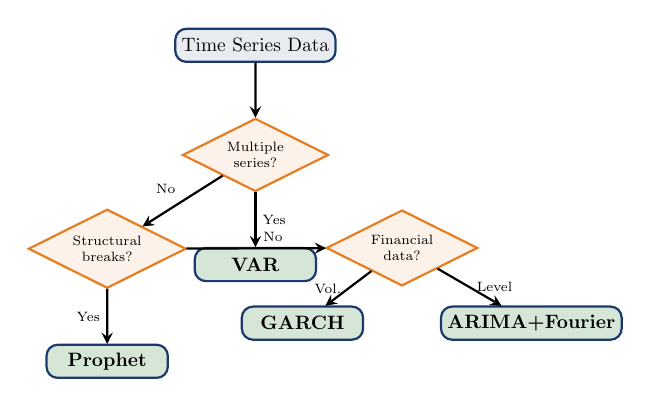
\begin{tikzpicture}[scale=0.7, transform shape,
        node distance=1cm,
        box/.style={rectangle, draw=MainBlue, thick, fill=MainBlue!10, rounded corners, minimum width=2.2cm, minimum height=0.6cm, align=center},
        decision/.style={diamond, draw=Orange, thick, fill=Orange!10, aspect=2, align=center, font=\scriptsize},
        arrow/.style={->, thick, >=stealth}
    ]
        \node[box] (start) {Time Series Data};
        \node[decision, below=of start] (q1) {Multiple\\series?};
        \node[decision, below left=1cm and 1.3cm of q1] (q2) {Structural\\breaks?};
        \node[decision, below right=1cm and 1.3cm of q1] (q3) {Financial\\data?};
        \node[box, fill=Forest!20, below=of q1] (var) {\textbf{VAR}};
        \node[box, fill=Forest!20, below=of q2] (prophet) {\textbf{Prophet}};
        \node[box, fill=Forest!20, below left=0.7cm and 0cm of q3] (garch) {\textbf{GARCH}};
        \node[box, fill=Forest!20, below right=0.7cm and 0cm of q3] (arima) {\textbf{ARIMA+Fourier}};
        \draw[arrow] (start) -- (q1);
        \draw[arrow] (q1) -- node[right] {\scriptsize Yes} (var);
        \draw[arrow] (q1) -- node[above left] {\scriptsize No} (q2);
        \draw[arrow] (q2) -- node[left] {\scriptsize Yes} (prophet);
        \draw[arrow] (q2) -- node[above right] {\scriptsize No} (q3);
        \draw[arrow] (q3) -- node[left] {\scriptsize Vol.} (garch);
        \draw[arrow] (q3) -- node[right] {\scriptsize Level} (arima);
    \end{tikzpicture}
    \end{center}
\end{frame}

\begin{frame}{Summary: Model Comparison}
    \begin{columns}[T]
        \column{0.55\textwidth}
        \begin{center}
        \footnotesize
        \begin{tabular}{llll}
            \toprule
            \textbf{Case} & \textbf{Challenge} & \textbf{Model} & \textbf{RMSE} \\
            \midrule
            Bitcoin & Volatility & GARCH & 2.14 \\
            Sunspots & Seasonality & Fourier & 29.68 \\
            Unemp & Break & Prophet & 0.42 \\
            Economic & Multi-var & VAR & 0.93 \\
            \bottomrule
        \end{tabular}
        \end{center}

        \column{0.45\textwidth}
        \begin{center}
            \includegraphics[width=\textwidth]{../charts/model_comparison.pdf}
        \end{center}
    \end{columns}

    \vspace{0.2cm}

    \begin{exampleblock}{Key Principle}
        \textbf{Match the model to the data characteristics.} No single model dominates---choose based on:
        \begin{itemize}
            \item Nature of the forecasting problem (level vs. volatility)
            \item Data properties (seasonality, breaks, multiple series)
            \item Interpretability requirements
        \end{itemize}
    \end{exampleblock}
\end{frame}

\begin{frame}{Comprehensive Model Comparison}
    \begin{center}
    \footnotesize
    \begin{tabular}{lcccc}
        \toprule
        \textbf{Feature} & \textbf{GARCH} & \textbf{Fourier} & \textbf{Prophet} & \textbf{VAR} \\
        \midrule
        \textbf{Target} & Volatility & Level & Level & Multiple \\
        \textbf{Seasonality} & No & Yes (long) & Yes (multi) & No \\
        \textbf{Structural breaks} & No & No & Yes & No \\
        \textbf{Multiple series} & No & No & No & Yes \\
        \textbf{Interpretable} & Medium & High & High & High \\
        \textbf{Parameters} & Few & $2K$ & Auto & Many \\
        \textbf{Missing data} & No & No & Yes & No \\
        \midrule
        \textbf{Best for} & Finance & Cycles & Business & Macro \\
        \bottomrule
    \end{tabular}
    \end{center}

    \vspace{0.3cm}

    \begin{columns}[T]
        \column{0.5\textwidth}
        \begin{block}{Our Results}
            \begin{itemize}
                \item GARCH: MAE=1.82 (volatility)
                \item Fourier: RMSE=29.68 (cycles)
                \item Prophet: RMSE=0.58 (breaks)
                \item VAR: Avg RMSE=0.93 (multi)
            \end{itemize}
        \end{block}

        \column{0.5\textwidth}
        \begin{exampleblock}{Key Insight}
            Each model excels in its domain. The art is matching the model to the data characteristics.
        \end{exampleblock}
    \end{columns}
\end{frame}

\begin{frame}{Best Practices for Applied Forecasting}
    \begin{columns}[T]
        \column{0.5\textwidth}
        \begin{block}{Methodology}
            \begin{enumerate}
                \item \textbf{Explore} data thoroughly
                \item \textbf{Test} for stationarity
                \item \textbf{Split} train/validation/test
                \item \textbf{Compare} models on validation
                \item \textbf{Report} test set metrics
            \end{enumerate}
        \end{block}

        \vspace{0.2cm}

        \begin{alertblock}{Common Mistakes}
            \begin{itemize}
                \item Peeking at test data
                \item Over-fitting to training set
                \item Ignoring model assumptions
                \item Not reporting uncertainty
            \end{itemize}
        \end{alertblock}

        \column{0.5\textwidth}
        \begin{exampleblock}{Practical Tips}
            \begin{itemize}
                \item Start simple (random walk, naive)
                \item Add complexity only if needed
                \item Visualize forecasts vs actuals
                \item Check residuals for patterns
                \item Report confidence intervals
            \end{itemize}
        \end{exampleblock}

        \vspace{0.2cm}

        \begin{block}{Remember}
            ``All models are wrong, but some are useful.'' \\
            \hfill --- George E. P. Box
        \end{block}
    \end{columns}
\end{frame}

%=============================================================================
% CONCLUSION
%=============================================================================
\begin{frame}{Key Takeaways}
    \begin{enumerate}
        \item \textbf{Rigorous Methodology}
        \begin{itemize}
            \item Train/validation/test split prevents overfitting
            \item Test set must remain untouched until final evaluation
        \end{itemize}

        \vspace{0.2cm}

        \item \textbf{Match Model to Data}
        \begin{itemize}
            \item Financial volatility $\rightarrow$ GARCH
            \item Long seasonality $\rightarrow$ Fourier terms
            \item Structural breaks $\rightarrow$ Prophet
            \item Multiple series $\rightarrow$ VAR
        \end{itemize}

        \vspace{0.2cm}

        \item \textbf{Interpret Results Carefully}
        \begin{itemize}
            \item Granger causality $\neq$ true causality
            \item Out-of-sample performance matters most
            \item Simpler models often work better
        \end{itemize}
    \end{enumerate}
\end{frame}

%=============================================================================
% REFERENCES
%=============================================================================
\begin{frame}{References}
    \footnotesize
    \begin{thebibliography}{99}
        \bibitem{box2015} Box, G.E.P., Jenkins, G.M., Reinsel, G.C., \& Ljung, G.M. (2015). \textit{Time Series Analysis: Forecasting and Control}. 5th ed., Wiley.

        \bibitem{hamilton1994} Hamilton, J.D. (1994). \textit{Time Series Analysis}. Princeton University Press.

        \bibitem{tsay2010} Tsay, R.S. (2010). \textit{Analysis of Financial Time Series}. 3rd ed., Wiley.

        \bibitem{hyndman2021} Hyndman, R.J., \& Athanasopoulos, G. (2021). \textit{Forecasting: Principles and Practice}. 3rd ed., OTexts.

        \bibitem{taylor2018} Taylor, S.J., \& Letham, B. (2018). Forecasting at Scale. \textit{The American Statistician}, 72(1), 37-45.

        \bibitem{bollerslev1986} Bollerslev, T. (1986). Generalized Autoregressive Conditional Heteroskedasticity. \textit{Journal of Econometrics}, 31(3), 307-327.

        \bibitem{sims1980} Sims, C.A. (1980). Macroeconomics and Reality. \textit{Econometrica}, 48(1), 1-48.
    \end{thebibliography}
\end{frame}

%=============================================================================
% DATA SOURCES
%=============================================================================
\begin{frame}{Data Sources}
    \begin{block}{Real Data Used in This Chapter}
        \begin{itemize}
            \item \textbf{Bitcoin}: Yahoo Finance (BTC-USD), 2019--2025
            \item \textbf{Sunspots}: Statsmodels Wolfer dataset, 1900--2008
            \item \textbf{US Unemployment}: Federal Reserve FRED (UNRATE), 2010--2025
            \item \textbf{Economic Variables}: FRED (GDPC1, UNRATE, CPIAUCSL, FEDFUNDS), 2000--2025
        \end{itemize}
    \end{block}

    \vspace{0.3cm}

    \begin{exampleblock}{Reproducibility}
        All analyses can be reproduced using the accompanying Jupyter notebook: \\
        \texttt{chapter10\_lecture\_notebook.ipynb}
    \end{exampleblock}
\end{frame}

%=============================================================================
% FINAL SLIDE
%=============================================================================
\begin{frame}[plain]
    \begin{tikzpicture}[remember picture, overlay]
        \fill[IDAred] (current page.north west) rectangle ([yshift=-0.15cm]current page.north east);
    \end{tikzpicture}

    \vfill
    \begin{center}
        {\Huge\textbf{\textcolor{MainBlue}{Thank You}}}\\[0.5cm]
        {\Large\textcolor{MediumGray}{Questions?}}\\[1cm]
        {\large Prof. Daniel Traian Pele, PhD}\\[0.2cm]
        {\texttt{danpele@ase.ro}}\\[0.5cm]
        {\footnotesize Bucharest University of Economic Studies}
    \end{center}
    \vfill

    \begin{tikzpicture}[remember picture, overlay]
        \fill[IDAred] (current page.south west) rectangle ([yshift=0.15cm]current page.south east);
    \end{tikzpicture}
\end{frame}

\end{document}
